\documentclass[aspectratio=169]{beamer}
\usetheme{Madrid}
\usecolortheme{default}

% Packages
\usepackage[utf8]{inputenc}
\usepackage{amsmath}
\usepackage{amssymb}
\usepackage{booktabs}
\usepackage{graphicx}
\usepackage{tikz}
\usetikzlibrary{shapes.geometric, arrows, positioning}

% Custom Color Palette (IIIT Bangalore Style)
\definecolor{IIITBBlue}{RGB}{0,51,102}
\definecolor{SlateGray}{RGB}{112,128,144}
\definecolor{DarkOrange}{RGB}{204,102,0}
\setbeamercolor{palette primary}{bg=IIITBBlue,fg=white}
\setbeamercolor{palette secondary}{bg=SlateGray,fg=white}
\setbeamercolor{palette tertiary}{bg=IIITBBlue,fg=white}
\setbeamercolor{titlelike}{parent=palette primary}
\setbeamercolor{structure}{fg=IIITBBlue}

% Title Slide Info
\title[Open-Set AI Generator Detection]{Open-Set AI-Generated Text Detection and Generator Rejection}
\subtitle{An Extension of the MAGE In-the-Wild AI Text Detection Framework}
\author[Wesley]{Student: B John Wesley (2022IMT-033)\\[0.2cm] Supervisor: Dr. Saswata Roy}
\institution[IIITB]{International Institute of Information Technology, Bangalore}
\date{August 2026}

\begin{document}

% Title Slide
\begin{frame}
\titlepage
\end{frame}

% Slide 2: Motivation
\begin{frame}{Motivation}
\begin{itemize}
    \item \textbf{Generalization Gap in AI Text Detection:} Most supervised AI detectors perform exceptionally well in "closed-lab" environments where training and test distributions match.
    \item \textbf{Failure in the Wild:} When deployed in real-world scenarios, these classifiers fail under distribution shifts (new domains or unseen generator architectures).
    \item \textbf{Closed-Set Attributor Limitations:} Existing supervised attribution systems operate under a closed-world assumption, forcing every machine-generated text into a known class (e.g., classifying a text as GPT or LLaMA even if it was generated by OPT).
    \item \textbf{Core Objective:} Implement a robust open-set rejection layer that models known generator distributions to detect and flag unseen generators as \textbf{UNKNOWN}.
\end{itemize}
\end{frame}

% Slide 3: Problem Statement
\begin{frame}{Problem Statement}
\begin{columns}
\begin{column}{0.5\textwidth}
    \textbf{Closed-Set Classification}
    \begin{itemize}
        \item Classifier is trained on class $A$ (GPT) and class $B$ (LLaMA).
        \item Test sample from class $C$ (OPT) is inputted.
        \item Model is \textbf{forced} to predict either $A$ or $B$ with high confidence, leading to false attributions.
    \end{itemize}
\end{column}
\begin{column}{0.5\textwidth}
    \textbf{Open-Set Classification (Proposed)}
    \begin{itemize}
        \item Classifier models known distributions of $A$ and $B$.
        \item Test sample from class $C$ (OPT) is inputted.
        \item Rejection layer measures the distance of the sample to the known distributions.
        \item Since the distance exceeds a validation-tuned threshold, the model predicts \textbf{UNKNOWN}.
    \end{itemize}
\end{column}
\end{columns}
\end{frame}

% Slide 4: The MAGE Research Paper (ACL 2024)
\begin{frame}{The MAGE Research Paper (ACL 2024)}
\begin{itemize}
    \item \textbf{Reference:} \textit{MAGE: Machine-generated Text Detection in the Wild} (ACL 2024) \cite{li-etal-2024-mage}.
    \item \textbf{Core Contribution:} MAGE establishes a comprehensive benchmarking framework to evaluate detectors under realistic distribution shifts.
    \item \textbf{Benchmark Design:}
    \begin{itemize}
        \item Covers multiple writing domains and LLM families.
        \item Examines \textbf{unseen-model} and \textbf{unseen-domain} settings.
        \item Tests robust detection under adversarial/paraphrased inputs.
    \end{itemize}
    \item \textbf{Key Finding:} Supervised classifiers suffer from severe performance drops when evaluated against unseen generator families, highlighting the need for structural open-set solutions.
\end{itemize}
\end{frame}

% Slide 5: What MAGE Means by "In the Wild"
\begin{frame}{What MAGE Means by ``In the Wild''}
The MAGE benchmark mimics real-world text verification by introducing three types of OOD shifts:
\begin{block}{1. Unseen Generator Shift}
Evaluating a detector trained on known generators (e.g., GPT-3.5) on text generated by a completely unseen generator (e.g., LLaMA, OPT).
\end{block}
\begin{block}{2. Unseen Domain Shift}
Evaluating a detector trained on news summaries on creative writing or informal forum discussions.
\end{block}
\begin{block}{3. Hybrid Shift}
Evaluating under simultaneous shifts in both domain and generator family, which represents the most realistic scenario.
\end{block}
\end{frame}

% Slide 6: MAGE Dataset \& Subsampling
\begin{frame}{MAGE Dataset \& Subsampling}
Our reproduction utilizes the official MAGE dataset, subsampled to optimize local execution:
\begin{itemize}
    \item \textbf{Three Writing Domains (Styles) Selected:}
    \begin{enumerate}
        \item \textbf{XSum (Extreme Summarization):} News summaries (factual, formal).
        \item \textbf{ELI5 (Explain Like I'm Five):} Forum Q\&A (informal, explanatory).
        \item \textbf{WritingPrompts:} Creative stories (highly descriptive, narrative).
    \end{enumerate}
    \item \textbf{Subsampled Configuration:}
    \begin{itemize}
        \item \textbf{Training set:} 15,000 balanced samples (5,000 per domain: 2,500 Human / 2,500 AI).
        \item \textbf{Validation set:} 1,872 balanced samples.
        \item \textbf{Test set:} 1,872 balanced samples.
    \end{itemize}
    \item \textbf{AI Generator Coverage:} Includes text generated by GPT, LLaMA, and OPT.
\end{itemize}
\end{frame}

% Slide 7: MAGE vs. My Implementation
\begin{frame}{MAGE vs. My Implementation}
\centering
\resizebox{0.9\textwidth}{!}{
\begin{tabular}{lll}
\toprule
\textbf{Aspect} & \textbf{Original MAGE Paper} & \textbf{My Implementation} \\
\midrule
\textbf{Objective} & Benchmark detection under OOD shifts & Reproduction + Open-set rejection layer \\
\textbf{Domains} & Broad multi-domain benchmark & XSum, ELI5, WritingPrompts subset \\
\textbf{Generators} & 27 LLM variants across families & GPT, LLaMA, OPT \\
\textbf{Primary PLM} & Longformer & DistilBERT \\
\textbf{Lexical} & FastText & FastText Baseline (TF-IDF + LR) \\
\textbf{Predictability} & GLTR & GLTR-style Rank Proportions \\
\textbf{Zero-Shot} & DetectGPT & DetectGPT-lite Perturbation Scorer \\
\textbf{OOD Setup} & Unseen model benchmarking & Explicit leave-one-generator-out rejection \\
\bottomrule
\end{tabular}
}
\end{frame}

% Slide 8: Supervised Baseline Results
\begin{frame}{Supervised Baseline Results}
The binary classifiers (Human vs. AI) were trained for 4 epochs on the subsampled MAGE dataset and evaluated on the test set:
\centering
\resizebox{0.8\textwidth}{!}{
\begin{tabular}{lccccc}
\toprule
\textbf{Model} & \textbf{Accuracy} & \textbf{AUC} & \textbf{Precision} & \textbf{Recall} & \textbf{F1-Score} \\
\midrule
FastText Baseline & 64.6\% & 0.711 & 67.1\% & 57.3\% & 0.618 \\
DistilBERT Classifier & \textbf{78.4\%} & \textbf{0.925} & \textbf{91.9\%} & \textbf{62.2\%} & \textbf{0.742} \\
\bottomrule
\end{tabular}
}
\begin{itemize}
    \item \textbf{Precision-Recall Trade-off:} The DistilBERT model is highly conservative (91.9\% precision), prioritizing the prevention of "false accusations" (labeling human text as AI) at the expense of recall (62.2\%).
    \item \textbf{Contextual Advantage:} The bidirectionality of DistilBERT captures syntactical and stylistic patterns far better than lexical n-grams (FastText).
\end{itemize}
\end{frame}

% Slide 9: Proposed Open-Set Novelty
\begin{frame}{Proposed Open-Set Novelty}
To address the closed-world attribution limitation, we introduce a \textbf{Two-Stage Forensic Pipeline}:
\begin{itemize}
    \item \textbf{Stage 1: Binary Detection}
    \begin{itemize}
        \item Analyzes incoming text to classify it as Human or Machine.
    \end{itemize}
    \item \textbf{Stage 2: Multi-Class Attribution \& Open-Set Rejection}
    \begin{itemize}
        \item If flagged as Machine, the text is routed to our open-set generator rejection layer.
        \item Calculates distance to the known generator embedding distributions (GPT and LLaMA).
        \item If the distance is below the threshold, it attributes the source to the closest class.
        \item If the distance exceeds the threshold, it rejects the text as \textbf{UNKNOWN} (unseen generator).
    \end{itemize}
\end{itemize}
\end{frame}

% Slide 10: Open-Set Rejection Pipeline
\begin{frame}{Open-Set Rejection Pipeline}
\centering
\resizebox{!}{0.75\textheight}{
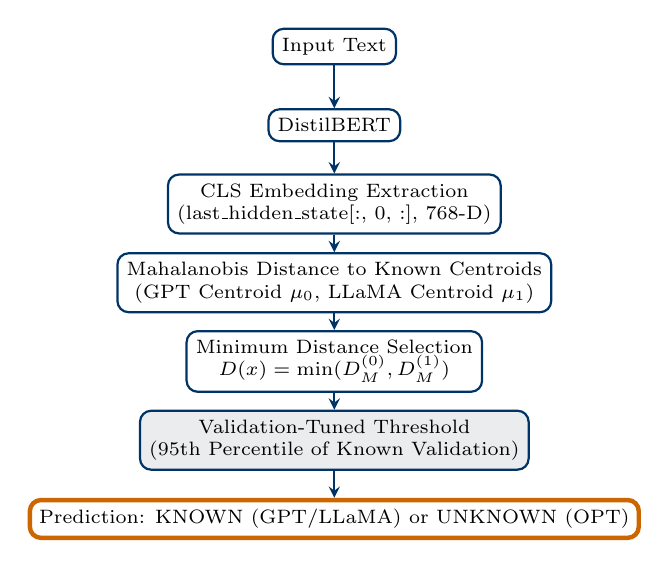
\begin{tikzpicture}[node distance=1.0cm, every node/.style={fill=white, draw=IIITBBlue, rounded corners, thick, align=center, font=\scriptsize}, arrow/.style={thick, ->, >=stealth, draw=IIITBBlue}]
\node (input) {Input Text};
\node (model) [below of=input] {DistilBERT};
\node (cls) [below of=model] {CLS Embedding Extraction\\(last\_hidden\_state[:, 0, :], 768-D)};
\node (dist) [below of=cls] {Mahalanobis Distance to Known Centroids\\(GPT Centroid $\mu_0$, LLaMA Centroid $\mu_1$)};
\node (min) [below of=dist] {Minimum Distance Selection\\$D(x) = \min(D_M^{(0)}, D_M^{(1)})$};
\node (thresh) [below of=min, fill=SlateGray!15] {Validation-Tuned Threshold\\(95th Percentile of Known Validation)};
\node (output) [below of=thresh, draw=DarkOrange, ultra thick] {Prediction: KNOWN (GPT/LLaMA) or UNKNOWN (OPT)};

\draw [arrow] (input) -- (model);
\draw [arrow] (model) -- (cls);
\draw [arrow] (cls) -- (dist);
\draw [arrow] (dist) -- (min);
\draw [arrow] (min) -- (thresh);
\draw [arrow] (thresh) -- (output);
\end{tikzpicture}
}
\end{frame}

% Slide 11: Mathematical Foundations
\begin{frame}{Mathematical Foundations}
\begin{block}{1. Class Centroids}
The mean embedding vector for each known class $c$ in the training set:
$$\mu_c = \frac{1}{N_c} \sum_{i=1}^{N_c} x_i^{(c)}$$
\end{block}
\begin{block}{2. Regularized Class Covariance}
Full covariance matrix computed over class training embeddings, adding diagonal regularization to prevent singularity:
$$\Sigma_c = \text{Cov}(X^{(c)}) + 10^{-4} \cdot I$$
\end{block}
\begin{block}{3. Minimum Mahalanobis Distance}
Measuring the OOD score of text embedding $x$ relative to the covariance-scaled known class distributions:
$$D(x) = \min_{c \in \{0, 1\}} \sqrt{(x - \mu_c)^T \Sigma_c^{-1} (x - \mu_c)}$$
\end{block}
\end{frame}

% Slide 12: Validation Threshold Selection
\begin{frame}{Validation Threshold Selection}
To prevent data leakage, the threshold is selected strictly before exposing the model to the unseen generator:
\begin{itemize}
    \item \textbf{Validation Set Profile:} Contains only known classes (500 GPT and 500 LLaMA validation samples).
    \item \textbf{Process:}
    \begin{enumerate}
        \item Feed the known validation samples through the fine-tuned model.
        \item Compute the minimum Mahalanobis distance for each validation sample.
        \item Select the \textbf{95th percentile} of these distances as the OOD threshold.
    \end{enumerate}
    \item \textbf{Zero-Leakage Guarantee:}
    \begin{itemize}
        \item The unseen generator (OPT) is completely absent during training, validation, centroid calculation, covariance calculation, and threshold selection.
        \item OPT is only loaded at the final step to evaluate unseen rejection rate.
    \end{itemize}
\end{itemize}
\end{frame}

% Slide 13: Baseline Open-Set Results (3A)
\begin{frame}{Baseline Open-Set Results (3A)}
\begin{columns}
\begin{column}{0.6\textwidth}
    \textbf{Baseline Parameters}
    \begin{itemize}
        \item Known generators: GPT + LLaMA
        \item Unseen generator: OPT
        \item Representation: CLS token
        \item Distance: Mahalanobis
    \end{itemize}
    \textbf{Observed Metrics}
    \begin{itemize}
        \item \textbf{Chosen Threshold:} 63.5972
        \item \textbf{Unseen OPT Rejection Rate:} \textbf{7.59\%} (608 / 8,012 OPT samples flagged)
        \item \textbf{Known Class False Rejection:} \textbf{3.90\%} (39 / 1,000 test samples incorrectly flagged)
        \item \textbf{OOD Score AUROC:} \textbf{0.6298}
    \end{itemize}
\end{column}
\begin{column}{0.4\textwidth}
    \begin{block}{Scientific Takeaway}
        The baseline performance represents a \textbf{modest} OOD separation capacity. While it maintains a low false rejection rate on known text, the system only detects a small fraction of the unseen OPT generator family.
    \end{block}
\end{column}
\end{columns}
\end{frame}

% Slide 14: Experiment 1: Representation Study
\begin{frame}{Experiment 1: Representation Study}
\textbf{Research Question:} How does the hidden state pooling method affect open-set generator rejection?
\centering
\resizebox{0.8\textwidth}{!}{
\begin{tabular}{lccc}
\toprule
\textbf{Metric} & \textbf{Baseline (CLS Pooling)} & \textbf{Experiment 1 (Mean Pooling)} & \textbf{Delta} \\
\midrule
\textbf{Unseen OPT Rejection} & \textbf{7.59\%} & \textbf{1.61\%} & -5.98\% \\
\textbf{Known False Rejection} & \textbf{3.90\%} & \textbf{4.40\%} & +0.50\% \\
\textbf{Open-Set OOD AUROC} & \textbf{0.6298} & \textbf{0.5251} & -0.1047 \\
\textbf{OOD Threshold} & 63.5972 & 5.8443 & -57.7529 \\
\bottomrule
\end{tabular}
}
\end{frame}

% Slide 15: Experiment 1 Interpretation
\begin{frame}{Experiment 1: Why Did Mean Pooling Perform Worse?}
\begin{block}{1. Classifier Alignment}
    Fine-tuning focuses the attribution gradients entirely on the \texttt{[CLS]} token. Other token representations do not capture global stylistic characteristics.
\end{block}
\begin{block}{2. Semantic Dominance}
    Mean pooling averages across all tokens. Because the texts share identical writing domains, semantic representations dominate and wash out generator style differences.
\end{block}
\end{frame}

% Slide 16: Experiment 2: Distance Metric Study
\begin{frame}{Experiment 2: Distance Metric Study}
\textbf{Research Question:} Does the choice of distance metric affect OOD generator rejection?
\centering
\resizebox{0.8\textwidth}{!}{
\begin{tabular}{lccc}
\toprule
\textbf{Metric} & \textbf{Baseline (Mahalanobis)} & \textbf{Experiment 2 (Cosine)} & \textbf{Delta} \\
\midrule
\textbf{Unseen OPT Rejection} & \textbf{7.59\%} & \textbf{0.85\%} & -6.74\% \\
\textbf{Known False Rejection} & \textbf{3.90\%} & \textbf{3.70\%} & -0.20\% \\
\textbf{Open-Set OOD AUROC} & \textbf{0.6298} & \textbf{0.4898} & -0.1400 \\
\textbf{OOD Threshold} & 63.5972 & 0.0158 & -63.5814 \\
\bottomrule
\end{tabular}
}
\end{frame}

% Slide 17: Experiment 2 Interpretation
\begin{frame}{Experiment 2: Why Did Cosine Distance Perform Worse?}
\begin{block}{1. Collinearity / Narrow Cone}
    DistilBERT fine-tuning results in embeddings that occupy a highly collinear cone. An angular distance (Cosine) of $\le 0.0158$ cannot isolate style details.
\end{block}
\begin{block}{2. Absence of Covariance Scaling}
    Cosine distance ignores how features vary and correlate. Mahalanobis distance scales the space using class covariances, highlighting stylistic variations.
\end{block}
\end{frame}

% Slide 18: Experiment 3: Generalization Study
\begin{frame}{Experiment 3: Generalization Study}
\textbf{Research Question:} Does the open-set rejection framework generalize to other unseen generator families?
\begin{itemize}
    \item We perform three independent leave-one-generator-out experiments.
    \item For each condition, we fine-tune a model and compute thresholds strictly excluding the held-out class.
    \item Separate training prevents information leakage and ensures strict OOD evaluation.
\end{itemize}
\end{frame}

% Slide 19: Experiment 3 Results
\begin{frame}{Experiment 3 Results}
\centering
\resizebox{0.85\textwidth}{!}{
\begin{tabular}{lccc}
\toprule
\textbf{Metric} & \textbf{3A: OPT unseen} & \textbf{3B: LLaMA unseen} & \textbf{3C: GPT unseen} \\
\midrule
\textbf{Known Generators} & GPT + LLaMA & GPT + OPT & LLaMA + OPT \\
\textbf{Unseen Generator} & OPT & LLaMA & GPT \\
\textbf{Threshold} & \textbf{5.9708} & \textbf{57.8356} & \textbf{72.8708} \\
\textbf{Unknown Rejection} & \textbf{1.41\%} & \textbf{5.12\%} & \textbf{27.85\%} \\
\textbf{Known False Rejection} & \textbf{4.10\%} & \textbf{6.40\%} & \textbf{5.80\%} \\
\textbf{OOD AUROC} & \textbf{0.5263} & \textbf{0.4919} & \textbf{0.7587} \\
\textbf{Unseen Samples} & 8,012 & 3,710 & 8,084 \\
\textbf{Known Samples} & 1,000 & 1,000 & 1,000 \\
\bottomrule
\end{tabular}
}
\end{frame}

% Slide 20: Domain-Wise OOD Results
\begin{frame}{Domain-Wise OOD Results}
The domain-wise OOD AUROC results for each leave-one-out configuration are presented below:
\centering
\resizebox{0.8\textwidth}{!}{
\begin{tabular}{lccc}
\toprule
\textbf{Unseen Generator} & \textbf{XSum AUROC} & \textbf{ELI5 AUROC} & \textbf{WritingPrompts AUROC} \\
\midrule
OPT (3A) & 0.5307 & 0.5340 & 0.4698 \\
LLaMA (3B) & 0.4555 & 0.3963 & 0.5609 \\
GPT (3C) & \textbf{0.6665} & \textbf{0.8006} & \textbf{0.7836} \\
\bottomrule
\end{tabular}
}
\begin{itemize}
    \item \textbf{Domain Divergence:} Open-set performance varies heavily across writing styles, with creative writing (WritingPrompts) and forum answers (ELI5) showing much stronger OOD separation for GPT than news articles (XSum).
\end{itemize}
\end{frame}

% Slide 21: Experiment 3 Interpretation
\begin{frame}{Experiment 3 Interpretation}
\begin{columns}
\begin{column}{0.5\textwidth}
    \textbf{Average Performance}
    \begin{itemize}
        \item Mean AUROC: \textbf{0.5923}
        \item Mean Unknown Rejection: \textbf{11.46\%}
        \item Mean Known False Rejection: \textbf{5.43\%}
    \end{itemize}
    \textbf{Generator Differences}
    \begin{itemize}
        \item \textbf{Easiest to Reject (GPT):} AUROC = \textbf{0.7587}.
        \item \textbf{Hardest to Reject (LLaMA):} AUROC = \textbf{0.4919}.
    \end{itemize}
\end{column}
\begin{column}{0.5\textwidth}
    \begin{block}{Scientific Interpretation}
        \begin{itemize}
            \item The open-set framework demonstrates \textbf{partial} generalization.
            \item GPT is highly separable because its closed-source, instruction-aligned training differs substantially from open-weights models.
            \item LLaMA and OPT show high overlap. The observed overlap may be related to similarities in learned representation distributions, model families, or training characteristics.
        \end{itemize}
    \end{block}
\end{column}
\end{columns}
\end{frame}

% Slide 22: Limitations \& Future Work
\begin{frame}{Limitations \& Future Work}
\begin{columns}
\begin{column}{0.5\textwidth}
    \textbf{Limitations}
    \begin{enumerate}
        \item \textbf{Limited Generator Scale:} Evaluated on only three generator families (GPT, LLaMA, OPT).
        \item \textbf{Modest Overall Performance:} Rejection rates for OPT and LLaMA are low.
        \item \textbf{Representation Collapse:} Fine-tuning shrinks feature variance, compressing Mahalanobis distance ranges.
    \end{enumerate}
\end{column}
\begin{column}{0.5\textwidth}
    \textbf{Future Work}
    \begin{enumerate}
        \item \textbf{Metric Learning:} Incorporate contrastive or triplet loss during fine-tuning to explicitly maximize OOD separation.
        \item \textbf{Generator Scaling:} Benchmark across a larger, more diverse set of LLM families.
        \item \textbf{Domain Robustness:} Evaluate the pipeline under joint cross-domain and cross-generator shifts.
    \end{enumerate}
\end{column}
\end{columns}
\end{frame}

% Slide 23: References
\begin{frame}[allowframebreaks]{References}
\footnotesize
\bibliographystyle{apalike}
\bibliography{presentation}
\end{frame}

\end{document}
